\documentclass[a4paper]{article}

\usepackage[utf8]{inputenc}
\usepackage[T1]{fontenc}
\usepackage{textcomp}
\usepackage[english]{babel}
\usepackage{amsmath, amssymb}


%figure support
\usepackage{import}
\usepackage{xifthen}
\pdfminorversion=7
\usepackage{pdfpages}
\usepackage{transparent}
\newcommand{\incfig}[1]{%
	\def\svgwidth{\columnwidth}
	\import{./figures/}{#1.pdf_tex}
}
\graphicspath{ {./figures/} }
\pdfsuppresswarningpagegroup=1

\begin{document}
\title{Message Integrity}
\author{Brandon Thompson}

	\section{Message Auth.\ Code}
	Goal: Integrity, no confidentiality.\\
	\textbf{Examples}
	\begin{itemize}
		\item Protecting public binaries on web
		\item Banner ads on webpages.
	\end{itemize}
	Generate tag: $S(k,m)\to $ tag\\
	Verify tag: $V\left( k,m,\text{tag} \right) =$ 'yes'\\
	Def: MAC $I=\left( S,V \right) $ defined over $\left( K,M,T \right) $ is a pair of algorithms:
	\begin{itemize}
		\item $S\left( k,m \right) $ outputs $t$ in $T$
		\item  $V\left( k,m,t \right) $ outputs 'yes' or 'no'.
	\end{itemize}
	
	Generate tag:\\
	$CRC\left( m \right) \to \text{tag}$ 
	\begin{itemize}
		\item Attacker can easily modify message $m$ and recompute CRC.
		\item CRC designed to detect \underline{random}, not malicious changes.
	\end{itemize}
	
	Attackers power: \ Chosen message attack\\
	for $m_1,m_2,\ldots,m_q$ attacker is given $t_i \leftarrow S\left( k_i,m_i \right) $ 
	%slide 6

	secure MAC size is $2^{80}$ 
	
	\section{Protecting System Files}
	At install time the system computes: $\left( \text{File is: }F_1, t_1=S\left( k,F_1 \right)  \right) , F_2,t_2,S\left( k,F_2 \right) $
	where k is derived from system password.\\

	\section{Secure PRF $\implies$ Secure MAC}
	For a PRF $F: K \times X \to Y$ define a MAC $I_F=\left( S,V \right) $ as:\\
	\begin{itemize}
		\item $S\left( k,m \right) := F\left( k,m \right) $
		\item $V\left( k, m, t \right): \text{output 'yes' if } t = F\left( k,m \right) \text{and 'no' otherwise.}$
	\end{itemize}
	Suppose $F:K \times  X \to Y$ is a secure PRF with $Y = \left\{ 0,1 \right\}^{10} $ \\
	Is the derived MAC I_F a secure MAC system?\\
	No tags are too short: anyone can guess the tag for any message. $Adv\left[ A,I_F \right] = \frac{1}{1024}$ 
	
	\section{CBC-MAC and NMAC}
	Recall that a secure PRF implies a secure MAC, as long as Y is large $S\left( k,m \right) = F\left( k,m \right) $ \\
	Given a PRF for short messages (AES), construct a PRF for long messages. From here on $X = \left\{ 0,1 \right\}^{n} $ where $n \approx 128$.\\
	The last encryption step in ECBC-MAC is because the MAC can be forged with one chosen message query:\\
	Suppose we define a MAC $I_{RAW} = \left( S,V \right) $ where 
	$S\left( k,m \right) = \text{rawCBC}\left( k,m \right) $. Then $I_{RAW}$ is easily broken 
	using a 1-chosen message attack. Adversary chooses and abritrary one block message $m \in X$.
	Requests tag for $m$. Get $t = F\left( k,m \right) $. Output $t$ as a MAC forgery for the 2-block
	message $\left( m, t \oplus m \right) $.
	\begin{center}
		$\text{rawCBC}\left( k,\left( m,t \oplus m \right)  \right) = F\left( k, F\left( k,m \right) \oplus \left( t\oplus m \right)  \right) = F\left( k,t \oplus \left( t \oplus m \right)  \right)  = t$
	\end{center}

	Theorem: For any L > 0, for every efficient q-query PRF advantage A attacking $F_{ECBC}$ or $F_{NMAC}$
	there exists an efficient adversary B s.t.:
	\begin{center}
		\[ Adv_{PRF}\left[ A, F_{ECBC} \right] \le Adv_{PRP}\left[ B, F \right] + \frac{2q^2}{|X|}\\
			Adv_{PRF}\left[ A, F_{NMAC} \right] \le  q \cdot L \cdot Adv_{PRF}\left[ B, F \right] + \frac{q^2}{2|K|} \] 
	\end{center}
	\\
	\\
	CBC-MAC is secure as long as $q \ll |X|^{\frac{1}{2}}$ \\
	NMAC is secure as long as $q \ll |K|^{\frac{1}{2}}\ \ \ \ \left( 2^{64}\text{for AES-128} \right)$.
	\subsection{Example}
	\begin{center}
		\[
		Adv_{PRF}\left[ A, F_{ECBC} \right] \le Adv_{PRP}\left[ B, F \right] + 2 \cdot \frac{q^2}{|X|}\\
		q = \# \text{messages MAC-ed with} k
		\] 
	\end{center}
	Suppose we want $Adv_{PRF}\left[ A,F_{ECBC} \right] \le \frac{1}{2^{32}} \Leftarrow \frac{q^2}{|X|}<\frac{1}{2^{32}}$
	\begin{itemize}
		\item AES: $|X| = 2^{128} \implies q<2^{48}$ So, after $2^{48}$ messages change key.
		\item 3DES: $|X| = 2^{64} \implies q<2^{16}$
	\end{itemize}
	\subsection{The Security Bounds are tight: an attack}
	After signing $|X|^{\frac{1}{2}}$ messages with ECBC-MAC or $|K|^{\frac{1}{2}}$ messages with NMAC
	the MACs become insecure.\\
	Suppose the underlying PRF $F$ is a PRP (e.g. AES)
	Then both PRFs (ECBC and NMAC) have the following extension property
			\begin{center}
				\[\forall x,y,w: F_{BIG}\left( k,x \right) = F_{BIG}\left( k,y \right)
					\implies
					F_{BIG}\left( k, x \| w \right) = F_{BIG}\left( k,y \| w \right) \\
				\] 
			\end{center}
	Let $F_{BIG}: K \times X \to Y$ be a PRF that has the extension property
	\begin{center}
		\[
			F_{BIG}\left( k,x \right) = F_{BIG}\left( k,y \right)
			\implies
			F_{BIG}\left( k,x\| w \right)  = F_{BIG}\left( k,y\|w \right)
		\] 
	\end{center}
	Generic attack on the derived MAC:
	\begin{enumerate}
		\item Issue $|Y|^{\frac{1}{2}}$ message queries for random messages in $X$. Obtain
			$\left( m_i,t_i \right) $ for $i = 1,\ldots, |Y|^{\frac{1}{2}}$ 
		\item Find a collision $t_u = t_v$ for $u\neq v$ (one exists w.h.p by birthday paradox)
		\item Choose some $w$ and query for $t:=F_{BIG}\left( k,m_u \| w \right) $ 
		\item Output forgery $\left( m_v\|w,t \right) $. Indeed $t:=F_{BIG}\left( k,m_v\|w \right) $
	\end{enumerate}
	\section{PMAC - parallel MAC}
	Suppose $P\left( k,i \right) $ is an easy to compute function, using keys $\left( k,k_1 \right) $
	and padding similar to CMAC. Let $F:K\times X \to X$ be a PRF. Define new PRF $F_{PMAC}:K^2\times X^{\le L}\to X$.
	Then the tag is calculated by xoring the message block and $P\left( k,i \right) $ and the output
	of that is put into the PRF $F\left( k_1,\cdot  \right) $ except for the last block.
	Every output of the PRF's is xored together and put into another PRF
	$F\left( k_1,\cdot  \right) $ to get the tag.
	\begin{figure}[ht]
		\centering
%		\incfig{pmac}
		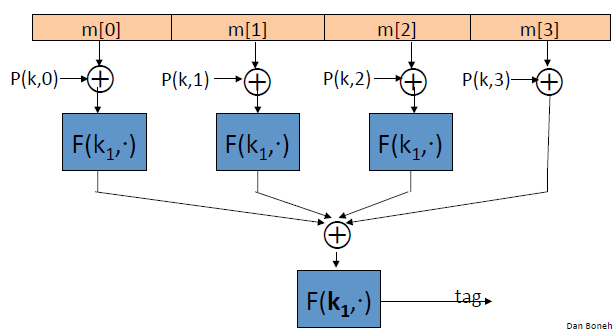
\includegraphics[width=0.8\textwidth]{pmac_slide}
		\caption{Parallel MAC taken from slides.}
		\label{fig:pmac}
	\end{figure}
	\subsection{PMAC is incremental}
	When $m\left[ 1 \right] \to m'\left[ 1 \right] $ can we quickly update the tag?
	\begin{center}
		\[
			\text{do } F^{-1}\left( k_1,tag \right) \oplus F\left( k_1,m\left[ 1 \right] \oplus P\left( k,1 \right)  \right) 
			\oplus F\left( k_1,m'\left[ 1 \right] \oplus P\left( k,1 \right)  \right)
		.\] 
	\end{center}
	Then apply $F\left( k_1,\cdot  \right) $ to receive the new tag.
	\section{One-time MAC}
	One-time MAC can be secure against \textbf{all} adversaries and faster than PRF-based MACs.
	Let $q$ be a large prime (e.g.\ $q = 2^{128}+51$ ). Key =
	$\left( a,b \right) \in \left\{ 1,\ldots,q \right\}^{2}$ (two random integers in $\left[ 1,q \right] $).
	Message = $\left( m\left[ 1 \right] ,\ldots, m\left[ L \right]  \right) $ where each block is 128 bit int.
	\begin{center}
		$S\left( \text{key, msg} \right) = P_{\text{msg}}\left( a \right) + b \left( \text{mod }q \right) $
	\end{center}
	where $P_{\text{msg}}\left( x \right)  = x^{L+1} + m\left[ L \right] \cdot x^L + \ldots + m\left[ 1 \right] \cdot x$ is a polynomial of degree $L+1$.\\
	we show: given $S\left( \text{key},\text{msg}_1 \right) $ adv.\ has no info about $S\left( \text{key},\text{msg}_2 \right) $.\\
	\subsection{One-time Security}
	Theorem: The one-time MAC satisfies  (L=msg-len)\\
	\[
		\forall m_1 \neq m_2,t_1,t_2:\ \ Pr_{a,b}\left[ S\left( \left( a,b \right) ,m_1 \right) =t_1
		\mid S\left( \left( a,b \right) ,m_2 \right) =t_2 \right] \le \frac{L}{q}
	\]
	Proof: $\forall m_1\neq m_2,t_1,t_2$ :
	\begin{enumerate}
		\item $Pr_{a,b}\left[ S\left( \left( a,b \right) ,m_2 \right) =t_2 \right] =Pr_{a,b}\left[ P_{m_2}\left( a \right) +b=t_2 \right] =\frac{1}{q} $
		\item $Pr_{a,b}\left[ S\left( \left( a,b \right) ,m_1 \right) =t_1 \text{ and } S\left( \left( a,b \right) ,m_2 \right) =t_2\right] =\\Pr_{a,b}\left[ P_{m_1}\left( a \right) -P_{m_2}\left( a \right) =t_1-t_2 \text{ and } P_{m_2}\left( a \right) +b=t_2 \right] \le \frac{L}{q^2}$
	\end{enumerate}
	$\implies$ given valid $\left( m_2,t_2 \right) $, adv.\ outputs $\left( m_1,t_1 \right) $ and is right with prob.\ $\le \frac{L}{q}$.

	\section{One-time MAC $\implies$ Many-time MAC}
	Let $\left( S,V \right) $ be a secure one-time MAC over $\left( K_l,M,\left\{ 0,1 \right\}^{n}  \right) $.\\
	Let $F:K_F \times \left\{ 0,1 \right\}^{n} \to \left\{ 0,1 \right\}^{n} $ be a secure PRF.\\
	\\
	\textbf{Carter-Wegman MAC:} $CW\left( \left( k_1,k_2 \right) ,m \right) = \left( r,F\left( k_1,r \right) \oplus S\left( k_2,m \right)  \right) $ for random $r \leftarrow \left\{ 0,1 \right\}^{n} $.\\
	Theorem: if $\left( S,V \right) $ is a secure \textbf{one-time} MAC and $F$ a secure PRF
	then $CW$ is a secure MAC outputting tags in $\left\{ 0,1 \right\}^{2n} $.\\
	How would you verify a CW tag $\left( r,t \right)$ on message $m$?\\
	Recall that $V\left( k_2,m,\cdot  \right) $ is the verification algorithm for the
	one time MAC.
\end{document}

